
\documentclass[a4paper, 10pt, twoside]{article}

\usepackage[top=1in, bottom=1in, left=1in, right=1in]{geometry}
\usepackage[utf8]{inputenc}
\usepackage[spanish, es-ucroman, es-noquoting]{babel}
\usepackage{setspace}
\usepackage{fancyhdr}
\usepackage{lastpage}
\usepackage{amsmath}
\usepackage{amsfonts}
\usepackage{amsthm}
\usepackage{verbatim}
\usepackage{fancyvrb}
\usepackage{graphicx}
\usepackage{float}
\usepackage{enumitem} % Provee macro \setlist
\usepackage{tabularx}
\usepackage{multirow}
\usepackage{hyperref}
\usepackage{xspace}
\usepackage{ulem} % Provee macro \uwave
\usepackage[toc, page]{appendix}


%%%%%%%%%% Constantes - Inicio %%%%%%%%%%
\newcommand{\titulo}{Trabajo Práctico 1}
\newcommand{\materia}{Bases de Datos}
\newcommand{\integrantes}{Delgado · Lovisolo · Petaccio · Rebecchi}
\newcommand{\cuatrimestre}{Segundo Cuatrimestre de 2014}
%%%%%%%%%% Constantes - Fin %%%%%%%%%%


%%%%%%%%%% Configuración de Fancyhdr - Inicio %%%%%%%%%%
\pagestyle{fancy}
\thispagestyle{fancy}
\lhead{\titulo · \materia}
\rhead{\integrantes}
\renewcommand{\footrulewidth}{0.4pt}
\cfoot{\thepage /\pageref{LastPage}}

\fancypagestyle{caratula} {
   \fancyhf{}
   \cfoot{\thepage /\pageref{LastPage}}
   \renewcommand{\headrulewidth}{0pt}
   \renewcommand{\footrulewidth}{0pt}
}
%%%%%%%%%% Configuración de Fancyhdr - Fin %%%%%%%%%%


%%%%%%%%%% Miscelánea - Inicio %%%%%%%%%%
% Evita que el documento se estire verticalmente para ocupar el espacio vacío
% en cada página.
\raggedbottom

% Separación entre párrafos.
\setlength{\parskip}{0.5em}

% Separación entre elementos de listas.
\setlist{itemsep=0.5em}

% Asigna la traducción de la palabra 'Appendices'.
\renewcommand{\appendixtocname}{Apéndices}
\renewcommand{\appendixpagename}{Apéndices}
%%%%%%%%%% Miscelánea - Fin %%%%%%%%%%


%%%%%%%%%% Macros para el modelo relacional - Inicio %%%%%%%%%%
\newcommand{\relacion}[3]{
  \noindent
  \textbf{#1}(\ignorespaces#2\unskip) \\
  #3
  \vspace{0.5em}
}
\newcommand{\pk}[1]{%
  \underline{#1}%
}
\newcommand{\fk}[1]{%
  \uwave{#1}%
}
\newcommand{\pkfk}[1]{%
  \pk{\fk{#1}}%
}
\newcommand{\clavespkck}[1]{
  PK = CK = \{#1\}
}
\newcommand{\clavespkckfk}[1]{
  PK = CK = FK = \{#1\}
}
\newcommand{\clavesfk}[1]{
  FK = \{#1\}
}
%%%%%%%%%% Macros para el modelo relacional - Fin %%%%%%%%%%

\begin{document}


%%%%%%%%%%%%%%%%%%%%%%%%%%%%%%%%%%%%%%%%%%%%%%%%%%%%%%%%%%%%%%%%%%%%%%%%%%%%%%%
%% Carátula                                                                  %%
%%%%%%%%%%%%%%%%%%%%%%%%%%%%%%%%%%%%%%%%%%%%%%%%%%%%%%%%%%%%%%%%%%%%%%%%%%%%%%%


\thispagestyle{caratula}

\begin{center}


\includegraphics[height=2cm]{DC.png} 
\hfill

\includegraphics[height=2cm]{UBA.jpg} 

\vspace{2cm}

Departamento de Computación,\\
Facultad de Ciencias Exactas y Naturales,\\
Universidad de Buenos Aires

\vspace{4cm}

\begin{Huge}
\titulo
\end{Huge}

\vspace{0.5cm}

\begin{Large}
\materia
\end{Large}

\vspace{1cm}

\cuatrimestre

\vspace{4cm}

\begin{tabular}{|c|c|c|}
\hline
Apellido y Nombre & LU & E-mail\\
\hline
Delgado, Alejandro N.  & 601/11 & nahueldelgado@gmail.com\\
Lovisolo, Leandro      & 645/11 & leandro@leandro.me\\
Petaccio, Lautaro José & 443/11 & lausuper@gmail.com\\
Rebecchi, Alejandro & 15/10 & alejandrorebecchi@gmail.com\\
\hline
\end{tabular}

\end{center}

\newpage


%%%%%%%%%%%%%%%%%%%%%%%%%%%%%%%%%%%%%%%%%%%%%%%%%%%%%%%%%%%%%%%%%%%%%%%%%%%%%%%
%% Introducción                                                              %%
%%%%%%%%%%%%%%%%%%%%%%%%%%%%%%%%%%%%%%%%%%%%%%%%%%%%%%%%%%%%%%%%%%%%%%%%%%%%%%%


\section{Introducción}

Presentaremos una solución para el problema de verificación y conservación de los resultados de las elecciones de los diferentes cargos políticos que presenta una universidad, tomando como guía, el estatuto de la Universidad de Buenos Aires \footnote{www.uba.ar/download/institucional/uba/9-32.pdf}.

El problema en cuestión contempla una serie de restricciones sobre como se realizan las votaciones y sobre quienes pueden presentarse para cada cargo que formarán parte de la verificación a modelar. Una vez resueltas las restricciones, se podrá validar los datos que se introduzcan, obteniendo registro de tanto los diferentes actores en las elecciones, como los cargos que tendrán los ganadores y para estos, los votos que recibieron, guardando quienes los realizaron solo para la elección que corresponda.

Utilizaremos las herramientas vistas en la materia, el modelado basado en el Diagrama de Entidad Relación, su MR resultante y la base de datos final que presentaremos en SQLite.


\newpage


%%%%%%%%%%%%%%%%%%%%%%%%%%%%%%%%%%%%%%%%%%%%%%%%%%%%%%%%%%%%%%%%%%%%%%%%%%%%%%%
%% Diagrama de Entidad Relación                                              %%
%%%%%%%%%%%%%%%%%%%%%%%%%%%%%%%%%%%%%%%%%%%%%%%%%%%%%%%%%%%%%%%%%%%%%%%%%%%%%%%


\section{Diagrama de Entidad Relación}

\subsection{Empadronado}
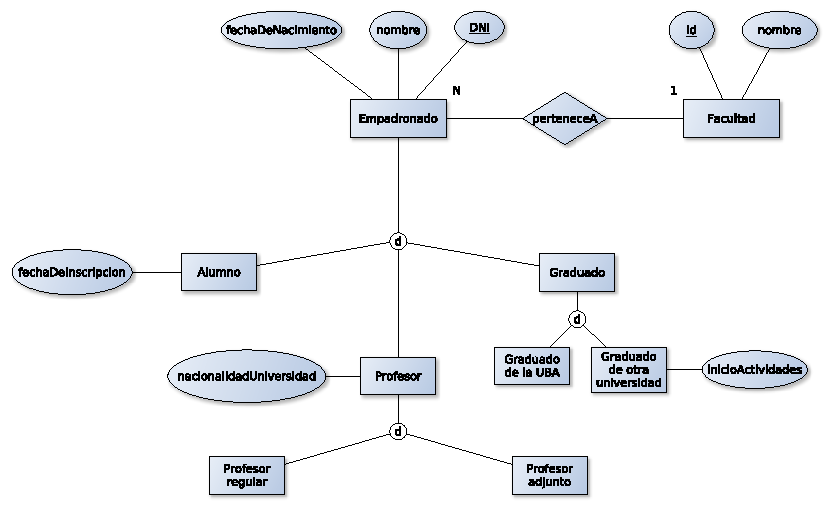
\includegraphics{../diagramas/empadronado.pdf}

\subsection{Elecciones Consejo Directivo}
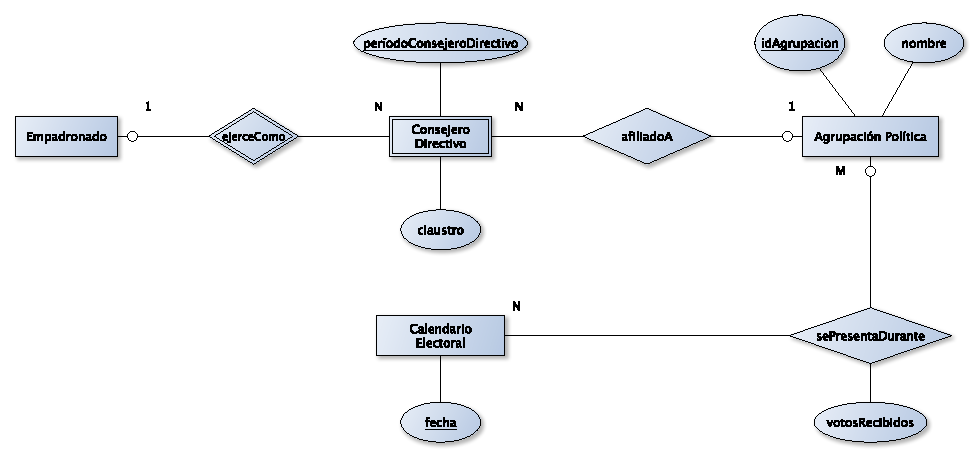
\includegraphics{../diagramas/eleccionesCD.pdf}

\subsection{Gobierno Superior}
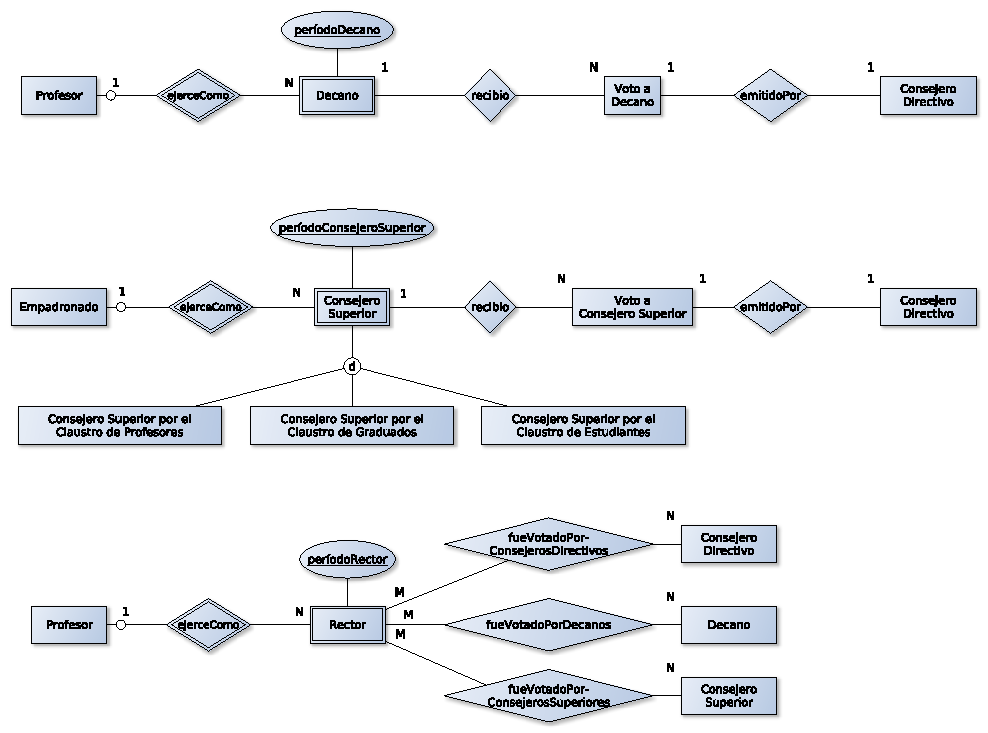
\includegraphics{../diagramas/gobiernoSuperior.pdf}


\subsection{Restricciones}


\subsubsection{Consejero Directivo}

\begin{itemize}
\item Para un periodo existen ocho representantes por los profesores, cuatro representantes por los graduados y cuatro representantes por los estudiantes.
%\item Para un periodo, la suma de la cantidad de votos en una fecha, no supera la cantidad de empadronados (?)
\item De los empadronados, solo profesores votan a consejeros directivos por el claustro de profesores
\item De los empadronados, solo estudiantes votan a consejeros directivos por el claustro de estudiantes
\item Solo pueden ser consejeros por el claustro de estudiantes, los estudiantes que tengan al menos un año desde la fecha de inscripcion
\item De los empadronados, solo graduados votan a consejeros directivos por el claustro de graduados
\item Si los graduados no son de la UBA, deben tener al menos un año de actividad para ser consejeros directivos
\item Solo votan consejeros directivos empadronados de la misma facultad
\item Un consejero directivo vota únicamente un decano durante su período, y el período del decano votado concuerda con el período del consejero
\item Un consejero directivo vota únicamente un consejero superior durante su período, y el período del consejero superior votado concuerda con el período del consejero
\end{itemize}


\subsubsection{Decano}

\begin{itemize}
\item Solo votan al decano consejeros directivos de la misma facultad
%\item Solo votan al decano consejeros directivos del último período registrado
\item Hay un decano por cada facultad por período
\item Los decanos deben haber tenido mayor o igual a 9 votos y menor o igual a 16
\end{itemize}


\subsubsection{Consejero Superior}

\begin{itemize}
\item Solo votan a consejeros superiores por el claustro de graduados, consejeros directivos por el claustro de graduados
\item Solo votan a consejeros superiores por el claustro de profesores, consejeros directivos por el claustro de profesores
\item Solo votan a consejeros superiores por el claustro de estudiantes, consejeros directivos por el claustro de estudiantes
%\item Solo votan a consejeros superiores, consejeros directivos del último período registrado
\item Solo pueden ser consejeros supueriores por el claustro de graduados, graduados
\item Solo pueden ser consejeros supueriores por el claustro de profesores, profesores
\item Solo pueden ser consejeros supueriores por el claustro de estudiantes, estudiantes
\item Existen por período, cinco representantes por el claustro de profesores, cinco por el de graduados y cinco por el de estudiantes
\end{itemize}


\subsubsection{Rector}

\begin{itemize}
\item Existen un solo rector por período
%\item Solo votan al rector, decanos, consejeros directivos y consejeros superiores del último período de cada uno
\item Obtuvo al menos la mitad más uno de los votos
\item Ser ciudadano argentino, tener edad mayor o igual que 30 y ser profesor
\end{itemize}


%%%%%%%%%%%%%%%%%%%%%%%%%%%%%%%%%%%%%%%%%%%%%%%%%%%%%%%%%%%%%%%%%%%%%%%%%%%%%%%
%% Modelo Relacional                                                         %%
%%%%%%%%%%%%%%%%%%%%%%%%%%%%%%%%%%%%%%%%%%%%%%%%%%%%%%%%%%%%%%%%%%%%%%%%%%%%%%%


\section{Modelo Relacional}


\relacion{Facultad}{
  \pk{idFacultad},
  nombre
}{
  \clavespkck{idFacultad}
}

\relacion{Empadronado}{
  \pk{DNI},
  nombre,
  fechaDeNacimiento,
  \fk{idFacultad},
  claustro
}{
  \clavespkck{DNI}
}

\relacion{Estudiante}{
  \pkfk{DNI},
  fechaDeInscripcion
}{
  \clavespkckfk{DNI}
}

\relacion{Graduado}{
  \pkfk{DNI},
  universidad
}{
  \clavespkckfk{DNI}
}

\relacion{Graduado de la UBA}{
  \pkfk{DNI}
}{
  \clavespkckfk{DNI}
}

\relacion{Graduado de otra universidad}{
  \pkfk{DNI},
  inicioActividades
}{
  \clavespkckfk{DNI}
}

\relacion{Profesor}{
  \pkfk{DNI},
  nacionalidadUniversidad
}{
  \clavespkckfk{DNI}
}

\relacion{Consejero Directivo}{
  \pk{\fk{DNI}, períodoConsejeroDirectivo},
  \fk{idAgrupación},
  claustro
}{
  \clavespkck{(DNI, períodoConsejeroDirectivo)} \\
  \clavesfk{DNI, idAgrupación}
}

\relacion{Consejero Directivo por el Claustro de Estudiantes}{
  \pkfk{DNI, períodoConsejeroDirectivo}
}{
  \clavespkckfk{(DNI, períodoConsejeroDirectivo)}
}

\relacion{Consejero Directivo por el Claustro de Graduados}{
  \pkfk{DNI, períodoConsejeroDirectivo}
}{
  \clavespkckfk{(DNI, períodoConsejeroDirectivo)}
}

\relacion{Consejero Directivo por el Claustro de Profesores}{
  \pkfk{DNI, períodoConsejeroDirectivo}
}{
  \clavespkckfk{(DNI, períodoConsejeroDirectivo)}
}

\relacion{Agrupación política}{
  \pk{idAgrupación},
  nombre
}{
  \clavespkck{idAgrupación}
}

\relacion{sePresentaDurante}{
  \pk{\fk{idAgrupación}, \fk{fecha}},
  votosRecibidos
}{
  \clavespkck{(idAgrupación, fecha)} \\
  \clavesfk{idAgrupación, fecha}
}

\relacion{Calendario Electoral}{
  \pk{fecha}
}{
  \clavespkck{fecha}
}

\relacion{Decano}{
  \pk{\fk{DNI}, períodoDecano}
}{
  \clavespkck{(DNI, períodoDecano)} \\
  \clavesfk{DNI}
}

\relacion{VotoADecano}{
  \pk{\fk{DNIDecano, períodoDecano},
      \fk{DNIConsejeroDirectivo, períodoConsejeroDirectivo}}
}{
  \clavespkck{(DNIDecano, períodoDecano, DNIConsejeroDirectitvo, períodoConsejeroDirectivo)} \\
  \clavesfk{(DNIDecano, períodoDecano), (DNIConsejeroDirectitvo, períodoConsejeroDirectivo)}
}

\relacion{Consejero Superior}{
  \pk{\fk{DNI}, períodoConsejeroSuperior},
  claustro
}{
  \clavespkck{(DNI, períodoConsejeroSuperior)} \\
  \clavesfk{DNI}
}

\relacion{Consejero Superior por el Claustro de Estudiantes}{
  \pkfk{DNI, períodoConsejeroSuperior}
}{
  \clavespkckfk{(DNI, períodoConsejeroSuperior)}
}

\relacion{Consejero Superior por el Claustro de Profesores}{
  \pkfk{DNI, períodoConsejeroSuperior}
}{
  \clavespkckfk{(DNI, períodoConsejeroSuperior)}
}

\relacion{Consejero Superior por el Claustro de Graduados}{
  \pkfk{DNI, períodoConsejeroSuperior}
}{
  \clavespkckfk{(DNI, períodoConsejeroSuperior)}
}

\relacion{VotoAConsejeroSuperior}{
  \pk{\fk{DNIConsejeroSuperior, períodoConsejeroSuperior},
      \fk{DNIConsejeroDirectivo, períodoConsejeroDirectivo}}
}{
  \clavespkck{(DNIConsejeroSuperior, períodoConsejeroSuperior, DNIConsejeroDirectivo períodoConsejeroDirectivo)} \\
  \clavesfk{(DNIConsejeroSuperior, períodoConsejeroSuperior), (DNIConsejeroDirectivo, períodoConsejeroDirectivo)}
}

\relacion{Rector}{
  \pk{\fk{DNI}, períodoRector}
}{
  \clavespkck{(DNI, períodoRector)} \\
  \clavesfk{DNI}
}

\relacion{fueVotadoPorConsejerosDirectivos}{
  \pk{\fk{DNIRector, períodoRector},
      \fk{períodoConsejeroDirectivo, DNIConsejeroDirectivo}}
}{
  \clavespkck{(DNIRector, períodoRector, DNIConsejeroDirectivo, períodoConsejeroDirectivo)} \\
  \clavesfk{(DNIRector, períodoRector), (DNIConsejeroDirectivo, períodoConsejeroDirectivo)}
}

\relacion{fueVotadoPorDecanos}{
  \pk{\fk{DNIRector, períodoRector},
      \fk{DNIDecano, períodoDecano}}
}{
  \clavespkck{(DNIRector, períodoRector, DNIDecano, períodoDecano)} \\
  \clavesfk{(DNIRector, períodoRector), (DNIDecano, períodoDecano)}
}

\relacion{fueVotadoPorConsejerosSuperiores}{
  \pk{\fk{DNIRector, períodoRector},
      \fk{DNIConsejeroSuperior, períodoConsejeroSuperior}}
}{
  \clavespkck{(DNIRector, períodoRector, DNIConsejeroSuperior, períodoConsejeroSuperior)} \\
  \clavesfk{(DNIRector, períodoRector), (DNIConsejeroSuperior, períodoConsejeroSuperior)}
}


\end{document}
